\ifmostrarGabarito
\textbf{Resposta: (B)}

\textbf{Justificativa:}
1. O comando \texttt{global taxa} declara que a função modificará a variável global \texttt{taxa}, atribuindo-lhe o novo valor \texttt{1.20}.
2. Como listas são objetos mutáveis passados por referência, a modificação \texttt{valores[i] = valores[i] * 1.20} altera diretamente os elementos da lista \texttt{precos}:
   - $10.0 \times 1.20 = 12.0$
   - $20.0 \times 1.20 = 24.0$
   Portanto, \texttt{precos} torna-se \texttt{[12.0, 24.0]}.
3. O somatório retornado é $12.0 + 24.0 = 36.0$.
4. A variável global \texttt{taxa} foi atualizada para \texttt{1.20}.
\else
\par\vspace{0.15cm}
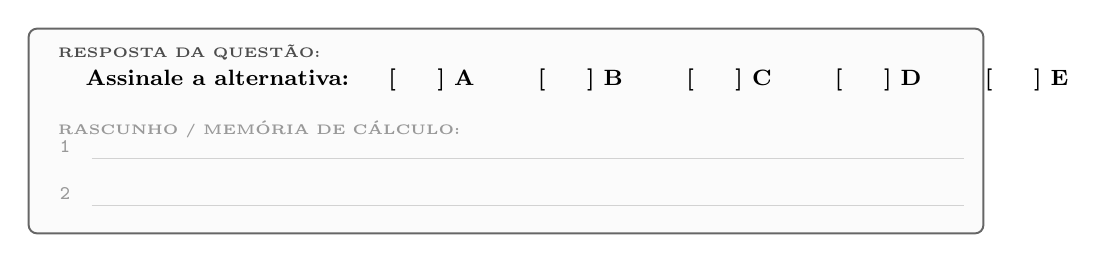
\begin{tikzpicture}
  \draw[rounded corners=3pt, draw=black!60, line width=0.7pt, fill=gray!3] (0,0) rectangle (\linewidth, -2.6cm);
  \node[anchor=north west, font=\tiny\bfseries\color{black!70}] at (0.25cm, -0.08cm) {RESPOSTA DA QUESTÃO:};
  \node[anchor=west, font=\footnotesize\bfseries] at (0.6cm, -0.65cm) {Assinale a alternativa: \quad [ \hspace{0.3cm} ] A \qquad [ \hspace{0.3cm} ] B \qquad [ \hspace{0.3cm} ] C \qquad [ \hspace{0.3cm} ] D \qquad [ \hspace{0.3cm} ] E};
  \node[anchor=north west, font=\tiny\bfseries\color{gray!80}] at (0.25cm, -1.05cm) {RASCUNHO / MEMÓRIA DE CÁLCULO:};
  \draw[gray!35, line width=0.4pt] (0.8cm, -1.65cm) -- (\linewidth-0.25cm, -1.65cm);
  \draw[gray!35, line width=0.4pt] (0.8cm, -2.25cm) -- (\linewidth-0.25cm, -2.25cm);
  \node[anchor=east, font=\scriptsize\ttfamily\color{gray!80}] at (0.65cm, -1.5cm) {1};
  \node[anchor=east, font=\scriptsize\ttfamily\color{gray!80}] at (0.65cm, -2.1cm) {2};
\end{tikzpicture}
\par\vspace{0.2cm}
\fi
